\section{Матричный калькулятор}
\subsection{Условие задания}
Создать приложение,  реализующее основные операции с векторами и матрицами:

\begin{enumerate}
    \item Ввод матрицы, вектора;
    \item Создание матриц (единичная, матрица как набор векторов);
    \item Умножение на число, вектор, матрицу;
    \item Сложение/вычитание двух матриц;
    \item Сложение/вычитание двух векторов;
    \item Скалярное и векторное произведение двух векторов;
    \item Транспонированная матрица;
    \item Определитель, ранг матрицы.
\end{enumerate}

Выводить сообщения об ошибках (ввод не числа, несоответствие размерностей)

\subsection{Теоретическая справка}
\subsubsection{Определение вектора}
Вектором называется направленный отрезок, для которого указаны его начало и конец. Свободный вектор --- множество одинаково направленных отрезков.

С точки зрения алгебры, вектор --- это строка или столбец матрицы.

Далее рассмотрим бинарные операции над векторами размерности $n \in \mathbb{N}$:
\begin{equation}
    \label{eq:vectors}
    \Vec{a} = \left(a_1, a_2, \dots, a_n\right),\;
    \Vec{b} = \left(b_1, b_2, \dots, b_n\right).
\end{equation}

\subsubsection{Алгебраическая сумма векторов}
Алгебраической суммой векторов (\ref{eq:vectors}) называют вектор:
\begin{equation}
    \Vec{a}+\Vec{b} = \left(a_1 + b_1, a_2 + b_2, \dots, a_n + b_n\right).
\end{equation}

\subsubsection{Произведения вектора и числа}
Произведением вектора $\Vec{a}$ (\ref{eq:vectors}) на число $\lambda \in \mathbb{R}$ называют вектор:
\begin{equation}
    \lambda\Vec{a} = \left(\lambda a_1, \lambda a_2, \dots, \lambda a_n\right).
\end{equation}

\subsubsection{Скалярное произведение векторов}
Скалярным произведением векторов $\Vec{a} \cdot \Vec{b}$ (\ref{eq:vectors}) называют число:
\begin{equation}
    \Vec{a} \cdot \Vec{b} = \left|\Vec{a}\right|\left|\Vec{b}\right|\cos\angle\left(\Vec{a},\,\Vec{b}\right).
\end{equation}

\subsubsection{Векторное произведение векторов}
Пусть $n = 3$ для векторов (\ref{eq:vectors}) --- из курса элементарной математики известно, что векторное произведение работает только в трёхмерном пространстве. Положим также, что векторы $\Vec{a}$ и $\Vec{b}$ не коллинеарны, то есть:
\begin{equation*}
    \exists\,i \in \mathbb{N}\cap\left[1,\,n\right]\;\forall\,\lambda\in\mathbb{N}\;a_i \neq \lambda b_i
\end{equation*}

Тогда векторным произведением называют вектор $\Vec{c}$ такой, что:
\begin{equation*}
    \begin{cases}
        \left|\Vec{c}\,\right| = S_{\Vec{a}\Vec{b}}, \\
        \Vec{c} \perp \Vec{a}, \\
        \Vec{c} \perp \Vec{b}, \\
        \left(\Vec{a},\,\Vec{b},\,\Vec{c}\right) - \textrm{правая тройка,}
    \end{cases}
\end{equation*}
где $S_{\Vec{a}\Vec{b}}$ --- площадь параллелограмма, построенного на $\Vec{a}$ и $\Vec{b}$ как на сторонах.

\subsection{Работа с матрицами}
\subsubsection{Определение матрицы}
Матрицей называют прямоугольную таблицу чисел.

Далее рассмотрим матрицы:
\begin{equation}
    \label{eq:matrix}
    A = \begin{pmatrix} a & b & c \\ d & e & f \\ g & h & i \\ \end{pmatrix}
\end{equation}

\subsection{Вид формы в конструкторе}
Форма имеет вид:

\begin{figure}
\centering
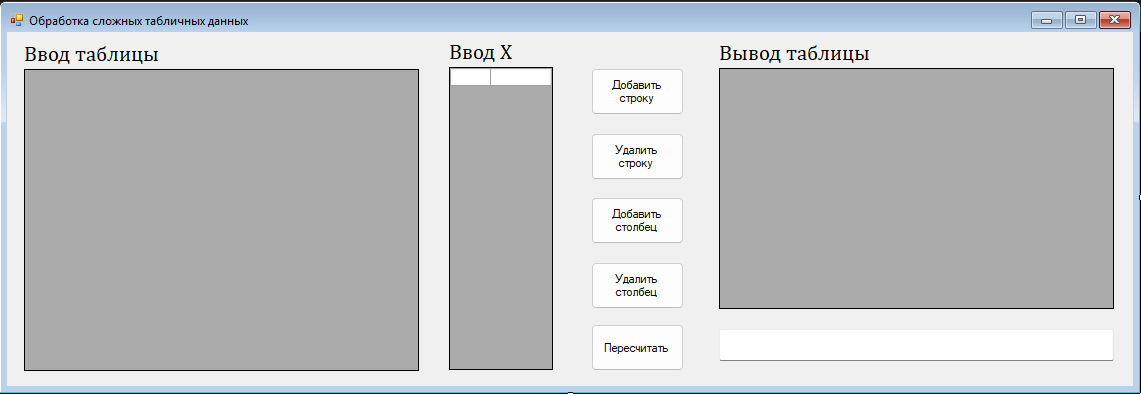
\includegraphics[width=0.5\linewidth]{images/handling-data-hard/form.png}
\caption{Форма окна для задания <<Простые вычисления>>}
\label{handling-data-hard-form}
\end{figure}

\subsection{Таблица с описанием элементов формы}
Все элементы формы были переименованы для большей читаемости. В таблице \ref{tab:handling-data-hard-form} представлены все изменения.

\begin{table}
\centering
\begin{tabular}{|m{0.3\textwidth}|m{0.3\textwidth}|m{0.3\textwidth}|}
\hline
\textbf{Описание элементов формы} & \textbf{Список изменённых атрибутов} & \textbf{Новое значение атрибута} \\
\hline
\hline
Окно формы & Text & Обработка сложных табличных данных \\
Метка <<Ввод таблицы>> & Name & tableInputLabel \\
Метка <<Ввод X>> & Name & xInputLabel \\
Метка <<Вывод таблицы>> & Name & outputLabel \\
Основная таблица ввода & Name & tableGrid \\
Дополнительная таблица ввода & Name & xGrid \\
Таблица вывода & Name & outputGridView \\
Поле для ошибок & Name & errorProvider \\
Кнопка <<Добавить строку>> & Name & addRow \\
Кнопка <<Удалить строку>> & Name & removeRow \\
Кнопка <<Добавить столбец>> & Name & addColumn \\
Кнопка <<Удалить столбец>> & Name & removeColumn \\
Кнопка <<Пересчитать>> & Name & executeButton \\

\hline
\end{tabular}
\caption{Значение атрибутов элементов в приложении для обработки табличных данных}
\label{tab:handling-data-hard-form}
\end{table}

\subsection{Примеры правильной и неправильной работы приложения}
При запуске приложения на экране появляется окно \ref{fig:handling-data-hard-start}.

\begin{figure}
\centering
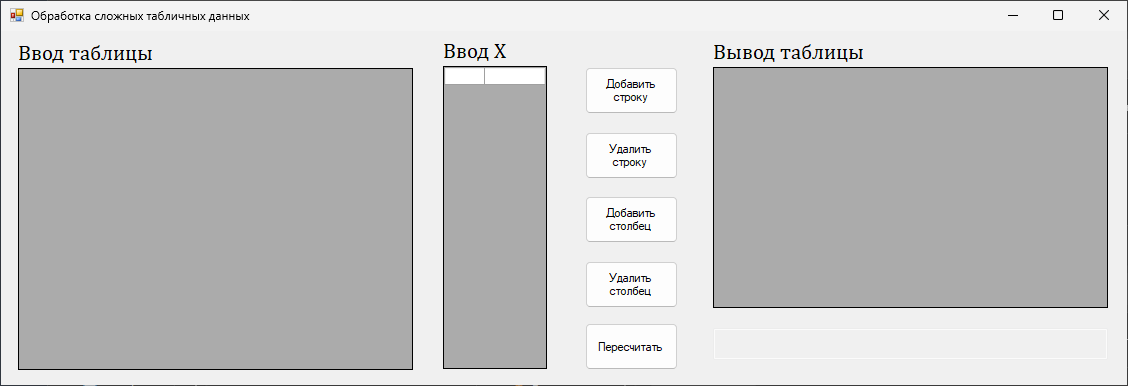
\includegraphics[width=0.5\linewidth]{images//handling-data-hard/start.png}
\caption{Запуск программы}
\label{fig:handling-data-hard-start}
\end{figure}

При нажатии на кнопку подсчитываются и подставляются значения в таблицу вывода. Также происходит обработка ошибок.

\begin{figure}
\centering
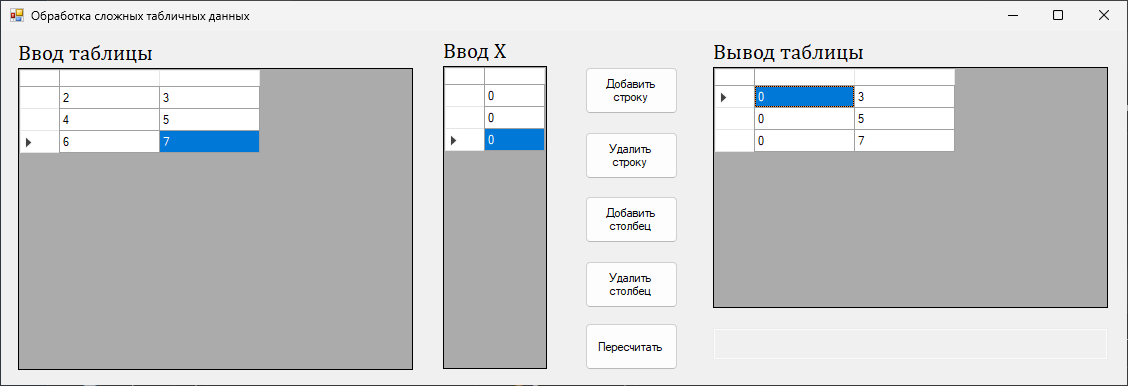
\includegraphics[width=0.5\linewidth]{images//handling-data-hard/okay.png}
\caption{Запуск с корректными данными}
\label{fig:handling-data-hard-okay}
\end{figure}

\begin{figure}
\centering
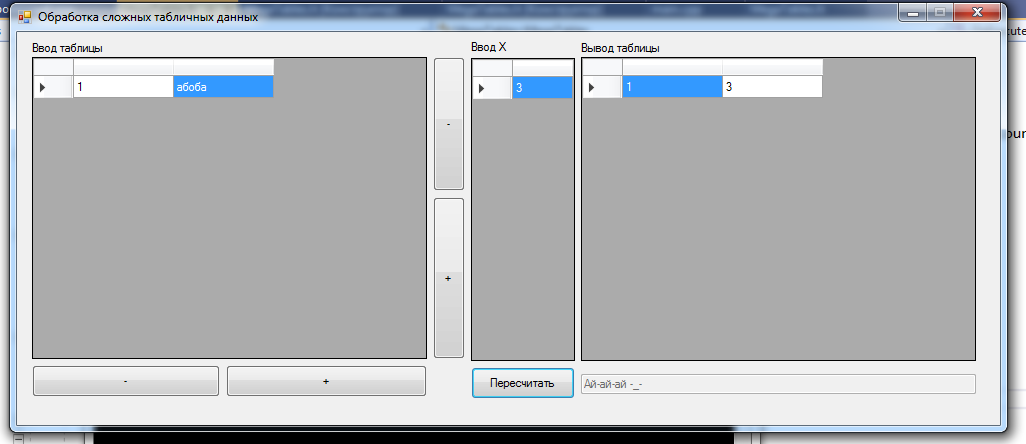
\includegraphics[width=0.5\linewidth]{images//handling-data-hard/error.png}
\caption{Пример ввода с некорректными данными}
\label{fig:handling-data-hard-error}
\end{figure}

\begin{figure}
\centering
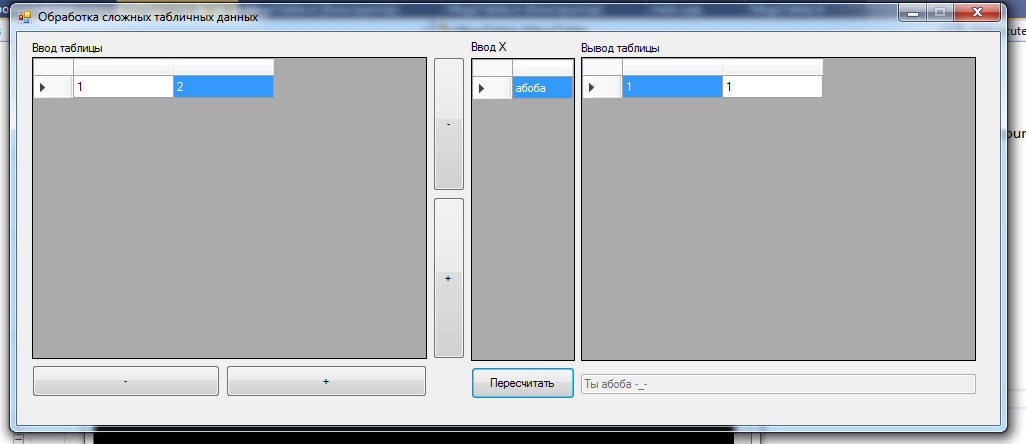
\includegraphics[width=0.5\linewidth]{images//handling-data-hard/error2.png}
\caption{Пример ввода с некорректными данными}
\label{fig:handling-data-hard-error2}
\end{figure}

\subsection{Примеры исходного кода}
\begin{minted}{cpp}

\end{minted}

Больше кода проекта доступно в приложении \ref{application-A}. Также в приложенном архиве можно найти полный код проекта.